\chapter{IMPROVED DUAL-SIM APPROACH TO GATESIM}
\label{chap:dualsim.tex}
Analyzing limitations associated with \emph{early dual-sim approach} shows that the main cause of inefficiency was the method used to capture, store, and applying test vectors onto the netlist. Analyzing limitations associated with \emph{co-sim approach}, it was inferred that the cause was bulky test-bench components associated with RTL simulations. Hence an improved solution would contain minimal testbench components retained and have an efficient method to capture, store, and apply test vectors. 

Test vectors are nothing but signal values at specific point in time. There are already different formats to store this information efficiently. FSDB \nomenclature{FSDB}{Fast Signal Database} is one such format. Hence it was suggested to improve gatesim methodology using FSDB itself as the format to store test vectors. The proposed solution should also improve on

\begin{description}
	\item[Storage requirements] Ensuring that storage resources are effectively used
	\item[Turn-around times] Should avoid re-build for different test vectors
\end{description}

FSDB\cite{SS:Verdi} or Fast Signal Database is a signal data file, similar to VCD\cite{ieee:v:2005} \nomenclature{VCD}{Value Change Dump} but much more compact. This format is in wide use across industry. Quick analysis revealed that FSDB as input test vectors could be accomplished. Existing API's \nomenclature{API}{Application Programming Interface} provided by Verdi\cite{SS:Verdi} tool set for FSDB format could be used to retrieve values from FSDB. PLI$/$VPI\cite{ieee:v:2005} could be used to drive stimulus onto netlist.


The improved methodology becomes a dual-simulation methodology with two separate simulations.
\begin{enumerate}
	\item First simulation with non-gatesim components to generate the test vectors in FSDB format.
	\item Second simulation with only gatesim components with capability to apply test vectors from FSDB directly.
\end{enumerate}



\section {DUAL-SIM FLOW}
In dual simulation approach the idea is to have two simulation but unlike co-sim not in parallel.  Instead here the simulations are separate from each other. We run the RTL simulation which will have test bench components for generating test vectors that will drive the inputs. This same test vectors are required for simulating the netlist environment. In cosimulation the same test bench will provide the stimulus to RTL and netlist. However in a dual simulation environment first RTL simulation will happen and the generated test vectors are stored in FSDB, which is used for simulating netlist. ~\figurename{~\ref{fig:gatesim_flow.eps}} gives the flow of proposed dual-sim approach.  
\begin{figure}[H]
\centering
\includegraphics[width=6in]{./figures/gatesim_flow.eps}
\caption{Dual Sim}
\label{fig:gatesim_flow.eps}
\end{figure}

Major steps involved in this flow are:

\begin{enumerate}
	\item Run RTL simulation

	RTL simulation is done along with test bench components for generating test vectors and verification. This is the same build for RTL verification stage. The simulation signals needs to be dumped into FSDB and for this the signal dump should be enabled during the run.
	\item As in the case of co simulation, Gatesim files need to be generated from input files obtained from LEC. Same infrastructure used in co-sim can be used for this.
	\item Get the gatesim build. Here the build structure will have the netlist and gatesim files only. RTL and the bulky testbench components are absent.
	\item Run simulation with specific FSDB file.
\end{enumerate}


\section{IMPLEMENTATION}
The implementation of the FSDB based dual simulation approach can be explained in three steps:
\begin{itemize}
\item How the FSDB file is generated.
\item Using FSDB dump files as test vector source.
\item Applying test vectors on to netlist.
\end{itemize}

\subsection{Generating test vector source file - FSDB file}
As discussed in previous section, the tests vectors for netlist simulation are same as the test vectors used for RTL simulation. These vectors are generated by testbench environment created for RTL simulation run. So the first step is to perform a standard RTL simulation with testbench components. These test benches will have various components for stimulus, assertion, debug feature etc. In this project we have used VSC Verilog simulator developed by Synopsys for RTL as well as net list simulation. 

{\bf VCS}: VCS is a high-performance, high-capacity Verilog simulator that  incorporates advanced, high-level abstraction verification  technologies into a single open native platform.VCS provides a fully featured implementation of the Verilog language as defined in the IEEE Standard Hardware Description Language Based on the Verilog Hardware Description Language (IEEE Std 1364-1995) and the Standard Verilog Hardware Description Language (IEEE Std 1364-2001). It supports most of the design and assertion constructs in SystemVerilog and PLI's for interface with other models, provides direct C kernel interface etc.  This is accepted as one of the fastest simulator when it comes to RTL verification. 

\subsubsection{RTL SIMULATION}

For RTL simulation the RTL sources and test bench files are compiled first and an executable file is generated for running the simulation. During the simulation VCS generate log files or reports giving details of the simulation. One feature provided by VCS is parallel FSDB dump. For this VCShave command to enable "{\emph dump}" during simulation run. This will dump all the {\emph signals} involved in RTL simulation and these FSDB dump files are used by waveform viewers as signal source.

\begin{figure}[H]
\centering
\includegraphics[width=4.5in, height=3.5in]{./figures/RTL_sim.eps}
\caption{RTL Simulation}
\label{fig:RTL_sim.eps}
\end{figure}



Once the RTL simulation completes with VCS signal dump option enabled, a .fsdb file is generated. This file is the vector source for netlist simulation. For each design and for each test condition, we need to perform dump enabled RTL simulation initially before going to netlist simulation. This is a onetime simulation from gate level verification point of view.


\subsection{USING FSDB AS TEST VECTORS}
Once the FSDB file is generated, next stage is extracting the signal values from this file and converting it into test vectors that can be applied for netlist simulation. Figure x shows the layout of programming infrastructure developed for this.

\begin{figure}[H]
\centering
<<<<<<< HEAD
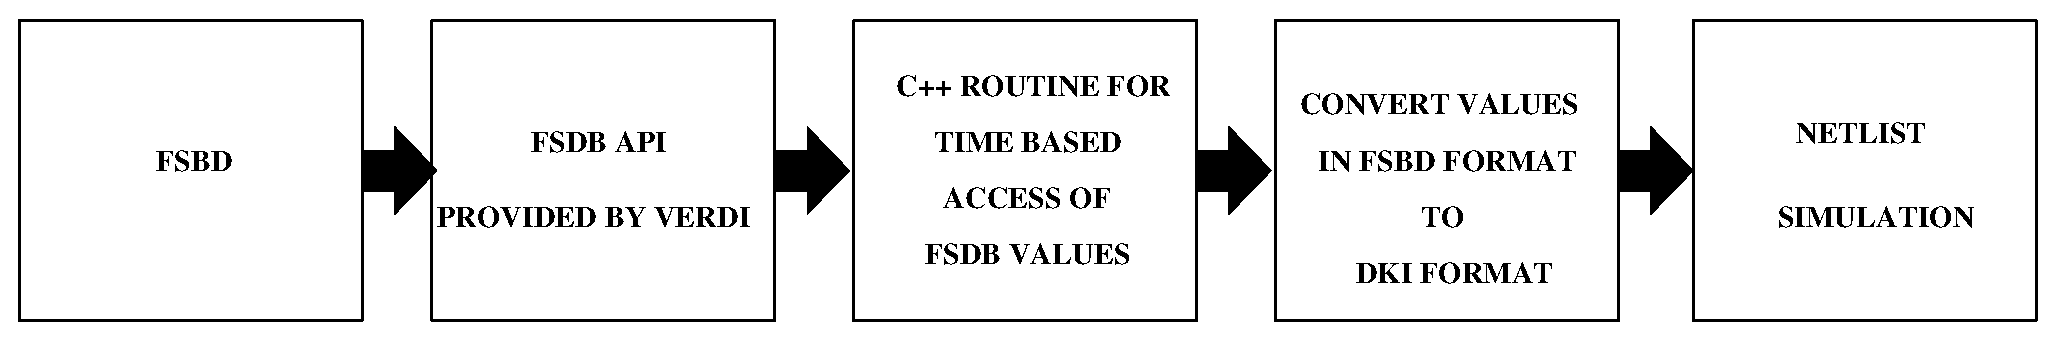
\includegraphics[width=5in, height=3in]{./figures/fsdb.eps}
=======
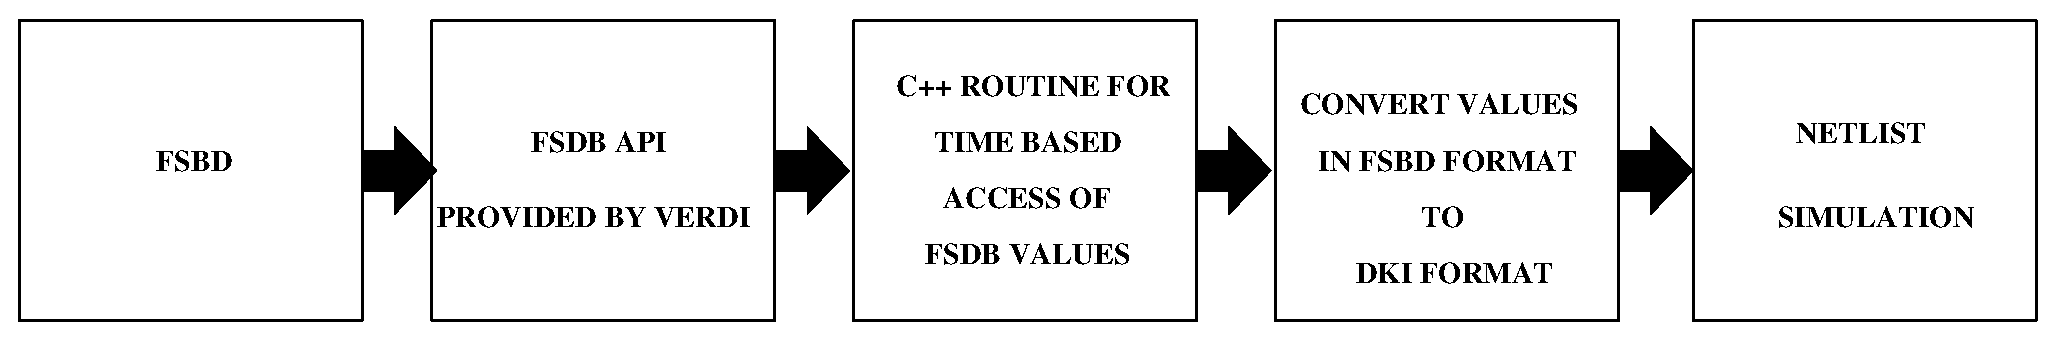
\includegraphics[width=5in, height=1.3in]{./figures/fsdb.ps}
>>>>>>> 67c22b93efe2b05d3738c447bedb04180afbaae5
\caption{Accessing FSDB Signals}
\label{fig:fsdb.eps}
\end{figure}

~\figurename{~\ref{fig:fsdb.eps}} shows how test vectors are obtained from .fsdb file and attached onto the netlist simulation flow. The various stages involved are explained below.

\paragraph{Extracting data from FSDB:}In FSDB signals are stored in binary format and can be accessed only by specific tools or using some appropriate APIs.  In this project we are using FSDB APIs provided by Verdi. These API's allow us to access each signal separately. 


\begin{figure}[H]
\centering
\includegraphics[width=4.5in, height=3.5in]{./figures/verdi.eps}
\caption{API For Accessing FSDB Signals}
\label{fig:verdi.eps}
\end{figure}






Once the list of RTL signals that need to be extracted is decided, make FSDB signals object handles corresponding to each signal. FSDB signal objects are also defined by the API and allow signals in FSDB file to be attached to these objects. Special "{\emph Attach()}" routines are provided for signal attach with objects.

However just attaching to the signal is not enough. A larger C++ infrastructure is required for accessing signals for gatesim because of the following reasons:
1.	Values contained in FSDB needs to be accessed in time-based fashion.
2.	Typical netlist contained hundreds of stimulus points with many wider bus-signals.
The C++ infrastructure will open the FSDB file and initiate a playback through the file. Whenever a signal that is attached using APIs changes, the C++ will identify this and will ensure the changed value is made available to the netlist simulation.  Figure x shows the complete flow of the C++ routine developed for FSDB signal access, conversion and application onto Verilog component.


\begin{figure}[H]
\centering
\includegraphics[width=6in]{./figures/cpp.eps}
\caption{C++ Routine for FSDB Signal Extraction}
\label{fig:cpp.eps}
\end{figure}




A set of RTL signal accessed at time based manner and applied onto netlist is effectively doing the job of test vectors as vectors are nothing but signal values at different instants of time.
Once signals are accessed from FSDB file by API's and C++ routine developed next step is applying it onto netlist. However Verilog based netlist cannot directly interact with extracted FSDB format objects. For this a conversion stage is required.  




\paragraph{Convert FSDB format to DKI format}: The FSDB format signals are converted to a standard format that can work with Verilog. There are many interfaces that allow Verilog-C interaction such as PLI, VPI (or PLI 2.0) or DKI. 
In this work we are using DKI which is an API that is supported only by VCS. This has the advantage of less simulation overhead and smaller memory footprint compared to VPI interface.
For converting FSDB signal format to DKI format, we are assigning signal values of the FSDB signal object to a corresponding DKI signal object. Similar to the creation of FSDB signal object list, create a DKI object list corresponding to the RTL signals. 

Whenever the C++ moves in time and identify a change in signal value in FSDB signal, an assign statement will assign the new FSDB signal value to DKI signal object.  These DKI signals can drive Verilog signals by using "{\emph Attach}" routine provided by API, that ties together DKI object with RTL signal. 

\subsection{NETLIST SIMULATION FLOW}
\begin{figure}[H]
\centering
\includegraphics[width=5in, height=3.5in]{./figures/netlist_sim.eps}
\caption{Netlist Simulation}
\label{fig:netlist_sim.eps}
\end{figure}

~\figurename{~\ref{fig:netlis_sim.eps}} show how test vectors are applied onto the netlist and how final comparison is done. Features of Improved gatesim methodology are:
\begin{enumerate}
	\item Obtain test vectors from FSDB; access it in time-based fashion.
	\item Drive stimulus onto a dummy RTL. This dummy RTL does not have any logic other than Input/output. All the input and output ports of the module netlist are included in this dummy RTL module. 
	\item Dummy RTL drives netlist stimulus and other stimulus points inside design (like fuses, un init flops).
	\item Apply appropriate force signals from FSDB directly on to the dummy RTL. The dummy RTL signal forces the netlist signals.
	\item Accomplish verification goals by cycle-comparing netlist behavior to that of its counterpart RTL (as available in the FSDB).
\end{enumerate}
It should be noted that the improved methodology is still dependent on vectors from RTL simulations and is not independent by itself. But gains obtained in turn-around times were of great benefit.



